\label{Chapter:distributions}

We have introduced the concepts of \emph{random variable},  \emph{random vector} and its \emph{probability distribution}. We will explain some concepts related to the latter ones.

\begin{ndef}
    The \emph{mode} of a distribution is the value at which the probability mass function takes its maximum value. That is, the value that is most likely to be sampled.
\end{ndef}

Distributions can be \emph{unimodal}, when their distribution has a single peak, \emph{bimodal} when their distribution has two peaks, and \emph{multimodal} when the number of peaks is equal or greater to $2$. 

\begin{nexample}
We can simulate the two following distributions:
\begin{enumerate}
    \item The distribution of the marks obtained in a test by the students of certain class.
    \item The distribution of the height of the plants from three different species.
\end{enumerate}
The result is the following:
\begin{figure}[H]%!htb]
    \minipage{0.45\textwidth}
      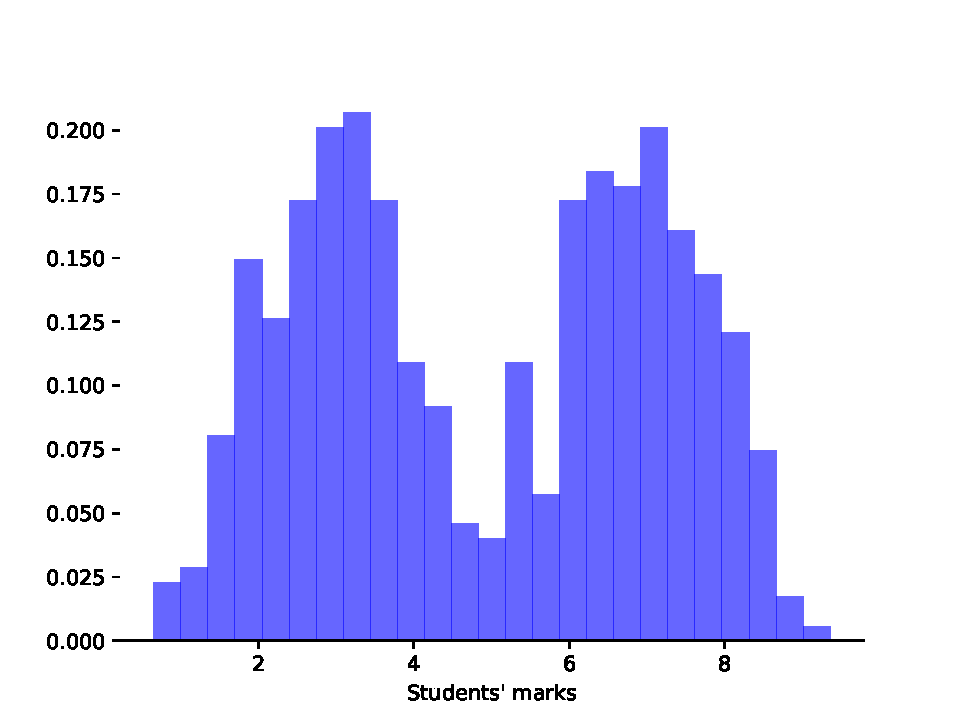
\includegraphics[width=\linewidth]{media/bimodal.pdf}
      \caption{Bimodal Distribution}\label{fig:linCM}
    \endminipage\hfill
    \minipage{0.45\textwidth}%
      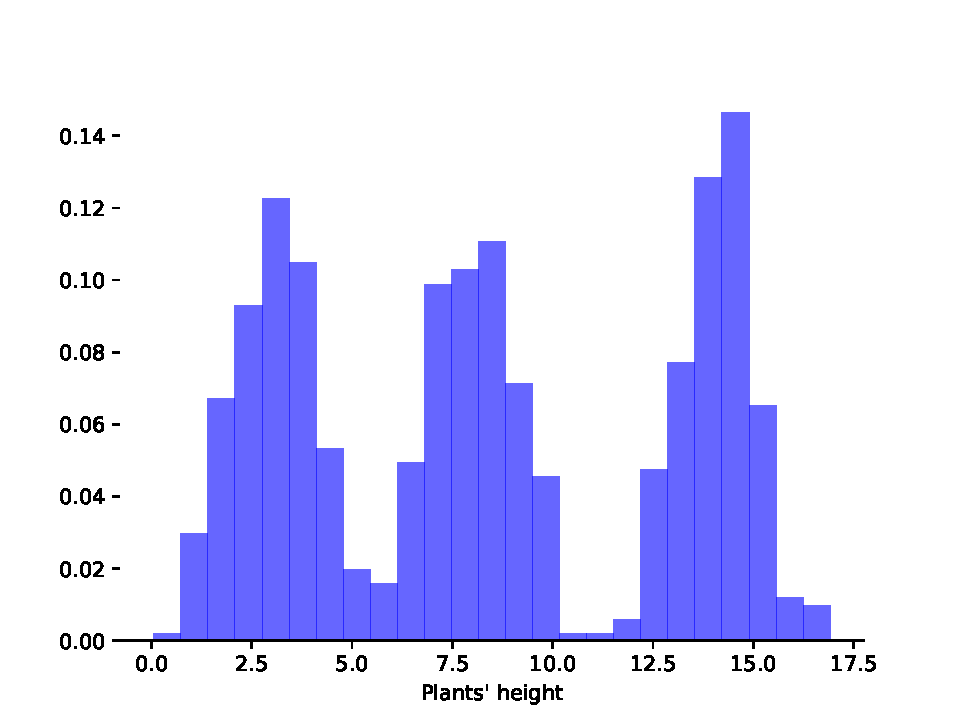
\includegraphics[width=\linewidth]{media/multimodal.pdf}
      \caption{Plants' height}\label{fig:RFCM}
    \endminipage
    \caption{Examples of bimodal and multimodal distributions.}
    \end{figure}
\end{nexample}


Now, given two distributions, we would like to determine how different they are from each other.
In order to compare them, we enunciate the definition of the Kullback-Leibler divergence.

\begin{ndef}
Let $P$ and $Q$ be probability distributions over the same probability space $\Omega$. Then, the Kullback-Leibler divergence is defined as:
$$
D_{KL}(P \ || \ Q) = E_P\left[\log{\frac{P(x)}{Q(x)}}\right].
$$
\end{ndef}
It is defined if, and only if, $P$ is \emph{absolutely continuous with respect to} $Q$, that is, if $P(A) = 0$ for any $A$ subset of $\Omega$ where $Q(A) = 0$.
 There are some properties of this definition that must be stated. 

\begin{nprop}
If $P,$ $Q$ are two probability distributions over the same probability space, then $D_{KL}(P|Q) \geq 0$.
\end{nprop}
\begin{proof}
Firstly, note that if $a \in \R^+$, then $\log \ a \leq a-1$. Then:
\begin{align*}
-D_{KL}(P \ || \ Q) & = - E_P\left[\log{\frac{P(x)}{Q(x)}}\right] \\
             & = E_P\left[\log{\frac{Q(x)}{P(x)}}\right] \\
             & \leq E_P\left[\left(\frac{Q(x)}{P(x)} - 1\right)\right]\\
             & = \int P(x) \frac{Q(x)}{P(x)} \mathop{dx} -1 \\
             & = 0.
\end{align*}
So we have obtained that $-D_{KL}(P\ ||\ Q) \leq 0$, which implies that $D_{KL}(P\ || \ Q) \geq 0$.
\end{proof}
As a corollary of this proposition, we can affirm that $D_{KL}(P\ ||\ Q)$ equals zero if and only if $P = Q$ almost everywhere. 
We will also remark the discrete case, as it will be used later. Let $P,Q$ be discrete probability distributions defined on the same probability space $\Omega$. Then, 
$$
D_{KL}(P\ ||\ Q) = \sum_{x \in \Omega} P(x) \log \left( \frac{P(x)}{Q(x)}\right).
$$

\section{Examples of distributions}

Let us present some examples o common distributions. They will be used further in this document.

\subsection*{Bernoulli}

Think for a moment that you want to model the possible outcomes of an experiment with two possibilites: sucess or failure. Imagine also that you already know that in your experiment there is a probability $p$ of 
achieving success. That is the intuitive idea of a Bernoulli distribution. We can define it more formally as follows: 

The \emph{Bernoulli distribution} is a discrete probability distribution of a random variable that takes two values, $\{0,1\}$, with probabilities $p$ and $q = 1-p$, respectively. We will say that our distribution is a $Bern(p)$.

If $k$ is a possible outcome, we can define
the probability mass function $f$ of a Bernoulli distribution as:
$$
f(k,p) = 
\begin{cases} 
p, \quad & \text{ if } k=1,\\
1-p, \quad & \text{ if } k = 0.
\end{cases}
$$
Using the expression of the mean for discrete random variables, we obtain that $E[X] = p$ and 
$$
\Var[X] = E[X^2] - E[X]^2 = E[X] - E[X]^2 = p-p^2 = p(1-p) = pq.
$$

As a note, this is just a particular case of the \emph{Binomial distribution} with $n=1$.

\subsection*{Gaussian Distribution}

The Gaussian (or normal) distribution is used to represent real-valued random variables whose distributions are not known.
Its importance relies in the fact that, using the \emph{central limit theorem}, we can assume that the average of many samples of
a random variable with finite mean and variance is a random variable whose distribution converges to a normal distribution as the number of samples increases.

\begin{ndef}
We say that the real valued random variable $X$ follows a \emph{normal distribution} of parameters $\mu,\sigma\in \R$ if, and only if,
its probability density function exists and it is determined by
\begin{equation}\label{gaussian:function}
f(x) = \frac{1}{\sigma \sqrt{2\pi}}e^{-\frac{1}{2}\left( \frac{x - \mu}{\sigma}\right)^2},
\end{equation}
where $\mu$ is the mean and $\sigma$ is its standard deviation. We denote this normal distribution as $X \sim \mathcal N (\mu,\sigma)$.
\end{ndef}

The particular case where $\mu = 0$ and $\sigma = 1$ is widely used in statistics. In this case, the density function is simpler:
\[
f(x) = \frac{1}{\sqrt{2\pi}}e^{-\frac{1}{2}x^2}.
\]

A remarkable property of these distributions is that, if $f : \R \to \R$ is a real-valued function defined 
as $f(x) = ax+b$, then $f(X) \sim \mathcal N (a\mu + b, \abs{a} \sigma)$.\\

In the same way that we extended random variables to random vectors, we can extend the normal distribution to a multivariate
random distribution.

\begin{ndef}
We say that a random vector $\bm{X} = (X_1,\dots,X_n)$ follows a multivariate normal distributions of parameters
$\mu \in \R^n$, $\Sigma \in \mathcal M_N(\R)$ if, and only if, its probabity density function is:
\begin{equation*}\label{gaussian:function}
f(x) = \frac{1}{\sqrt{\det(2\pi \Sigma)}}e^{-\frac{1}{2}(x - \mu )^T \Sigma^{-1} (x-\mu)}.
\end{equation*}
It is denoted $X \sim \mathcal N(\mu, \Sigma)$.
In this case, $\mu$ is the mean vector of the distribution and $\Sigma$ denotes the covariance matrix.  
\end{ndef}
